\documentclass[conference]{IEEEtran}
\IEEEoverridecommandlockouts
\usepackage{cite}
\usepackage{amsmath,amssymb,amsfonts}
\usepackage{algorithmic}
\usepackage{algorithm}
\usepackage{graphicx}
\usepackage{textcomp}
\usepackage{xcolor}
\usepackage{booktabs}
\usepackage{multirow}
\usepackage{float}
\usepackage{url}

% --- TIKZ SETUP ---
\usepackage{tikz}
\usepackage{pgfplots}
\pgfplotsset{compat=1.17}
\usetikzlibrary{shapes.geometric, arrows, positioning, fit, calc, backgrounds, er}

% --- DOCUMENT SETTINGS ---
\renewcommand{\baselinestretch}{1.0} 
\setlength{\parskip}{0em}
\setlength{\textfloatsep}{10pt}

\def\BibTeX{{\rm B\kern-.05em{\sc i\kern-.025em b}\kern-.08em
    T\kern-.1667em\lower.7ex\hbox{E}\kern-.125emX}}

\begin{document}

% ==========================================
% TITLE
% ==========================================
\title{NLOS Acoustic Sensing via Spectral Gating and GCC-PHAT}

% ==========================================
% AUTHOR & AFFILIATION
% ==========================================
\author{
\IEEEauthorblockN{
Polisetti Narendra\IEEEauthorrefmark{1}, 
Vijaya Raju Motru\IEEEauthorrefmark{2}, 
Suresh Kumar Sreedharan\IEEEauthorrefmark{3}, 
Praveena Mallampalli\IEEEauthorrefmark{4}, \\
T Murali Mohan\IEEEauthorrefmark{5}, and
T V Satyasheela\IEEEauthorrefmark{6}
}
\IEEEauthorblockA{\textit{Department of CSE, Swarnandhra College of Engineering and Technology}\\
Narasapur, Andhra Pradesh, India \\
\IEEEauthorrefmark{1}ORCID: 0009-0002-6355-138X, narendresh@yahoo.com \\
\IEEEauthorrefmark{2}vijayaraju.m@gmail.com, 
\IEEEauthorrefmark{3}ORCID: 0000-0001-9912-5927, nice.ssk@gmail.com \\
\IEEEauthorrefmark{4}praveena.iduri@gmail.com, 
\IEEEauthorrefmark{5}drtmm512@gmail.com, 
\IEEEauthorrefmark{6}satyasheela0506@gmail.com}
}

\maketitle

% ==========================================
% ABSTRACT
% ==========================================
\begin{abstract}
There are areas in many indoor situations where optical detection cannot indicate in time. The deployment of cameras in areas with bends, architectural junctions and partly occluded space generates permanent blind spots. The phenomenon of sound propagating and diffracting everywhere could offer a possible new physical modality.

The proposed work designs a deterministic acoustic sensor unit to detect high-decibel impulse events occurring at sources hidden by visual obstruction from corridor locations. Input audio signals are processed using a finite-size circular RAM buffer, which is immune to swap persistence attacks. An STFT-based spectral gating system is used to filter broadband impulse signals, whereas an autocorrelation-based periodicity filtering function eliminates any periodic mechanical signal artifacts. GCC-PHAT is employed in the directional analysis process for reverberating corridors in a well-defined reverberant field operational mode ($\mathcal{R}_{rev}$).

In controlled corridor evaluation, detection probability of more than 95\% was achieved within a 15 m safety envelope and end-to-end latency remained below about 120 ms.  Raw PCM segments are overwritten right after feature extraction. Hence, the light-weight directional metadata is all that is retained. The results show that one can use physics-driven acoustic processing to extend spatial awareness into non-line-of-sight environments under bounded latency and bounded audio retention.
\end{abstract}

\begin{IEEEkeywords}
Reverberant Acoustic Sensing, Non-Line-of-Sight Detection, Spectral Gating, GCC-PHAT Localization, Bounded-Memory Edge Processing, Deterministic Signal Discrimination.
\end{IEEEkeywords}

% ==========================================
% I. INTRODUCTION
% ==========================================
\section{Introduction}

The dominant thesis of this paper is that \textbf{deterministic signal-processing pipelines can reliably detect impulsive NLOS anomalies under reverberant corridor conditions while preserving bounded latency and bounded retention behavior}.

\subsection{Spatial Blindness in Line-of-Sight Monitoring}
The optical perception in indoor settings is intrinsically limited due to line-of-sight geometry constraints. Bends and junctions in corridors automatically lead to visual obstruction. It is impossible for cameras to cover all possible blind areas, while acoustic diffraction operates on a different domain than visual perception. NLOS perception is achieved via wave behavior, not imaging.

Acoustic sensing provides an alternative physical modality. Sound propagates omnidirectionally and diffracts around physical obstacles. In enclosed corridors, reflections from rigid surfaces extend acoustic reach well beyond visual coverage.

\subsection{Subsystem Scope and Canonical Separation}
This subsystem exists SOLELY for impulsive acoustic anomaly detection, directional metadata estimation, bounded-latency operation, and periodic mechanical noise filtering. It restricts audio storage operationally in the context of acoustic processing. This subsystem does NOT define immutable privacy policy , activate governance coordination , handle cryptographic provenance , establish runtime verifiability theorems , or understand semantically audio.

\subsection{Operational Constraints in Reverberant Corridors}
The use of acoustic sensing in indoor corridor environments comes with various limitations. Large and long corridors built using painted concrete, vinyl tile, and hard ceilings tend to cause multipath reflection effects. In such an environment, multipath reverberations usually exceed direct path energy beyond a few meters \cite{b25}.

Amplitude-based triggering is usually not very effective in such scenarios. Sound bursts produced by mechanical mechanisms, falling objects, or any form of sudden impact often surpass preset thresholds. TDOA-based positioning deteriorates due to echoes that arrive after a delay.

On the other hand, deep learning acoustic event detection models have some inherent drawbacks. For instance, AST models need to consider multi-second context windows and allocate adequate memory resources for inference. In cases where real-time detection is necessary, buffering multi-second chunks of audio data before inference cannot be achieved within 150 ms \cite{b26}.

However, the acoustic sensing unit described below follows a different methodology. Instead of classification of semantic content, it implements physical signal distinction on a local basis inside a circular RAM buffer. Derived characteristics, such as energy ratio, periodicity measure, and azimuth angle, are preserved, while PCM data samples are erased right away, adhering to privacy-by-design principles \cite{b32}, spatial cloaking methodologies \cite{b21}, and IoT privacy architectures \cite{b33}.

\subsection{Contributions}
The system is designed with respect to latency and storage issues. It utilizes only deterministic signal processing, and not any machine learning techniques. The key components are:
\begin{itemize}
    \item A formal definition of a reverberant-field operating regime, $\mathcal{R}_{rev}$, aligned with corridor geometries where the safety envelope substantially exceeds the acoustic critical distance.
    \item A two-stage filtering architecture combining spectral discrimination ($\delta$) and periodicity rejection ($\rho$) to suppress mechanical false positives.
    \item A latency-bounded GCC-PHAT implementation for azimuth estimation under multipath-dominant conditions.
    \item Empirical validation across staged and RIR-convolved corridor datasets demonstrating high detection rates within a 15 m non-line-of-sight radius.
\end{itemize}

The detection model does not attempt semantic audio interpretation. Its scope is deliberately narrower: detect high-energy, chaotic impulses and estimate their direction within bounded processing time.

% ==========================================
% II. RELATED WORK
% ==========================================
\section{Related Work}

Foundational work on privacy in video surveillance \cite{b1} has driven interest in audio surveillance \cite{b2} as an alternative modality \cite{b4}.

\subsection{Deep Learning AED vs. Edge Signal Processing}

The latest systems for detecting acoustic events depend on deep neural architectures designed for doing semantic sound classification \cite{b8, b12}. Architectures such as PANNs \cite{b22}, AST \cite{b23}, and convolutional audio classification backbones \cite{b35} can achieve strong performance on the FSD50K benchmark \cite{b19}, building on classical speech recognition \cite{b11} and time-frequency wavelet analysis \cite{b10}. These systems run on mel-spectrogram patches often spanning a few seconds.

When you have larger temporal context windows, they help enhance your performing semantic recognition accuracy but at the same time introduce structural latency. Introducing 10-second windows before inference is inherently against strict response constraints. Furthermore, large transformer-based models, such as those containing around 85 million parameters, require excessive memory and bandwidth \cite{b15, b16}. These models are particularly onerous on edge hardware based on ARM that does not contain NPU. Edge deployment feasibility remains constrained by memory-transfer and latency characteristics of embedded platforms. Prior analytical modeling of these constraints is available in \cite{b34}, while the present work focuses on reverberant acoustic sensing.

Safety applications have a different goal from those used for environmental classification or strain monitoring. In safety, early detection of high energy events is required. Deterministic signal processing is therefore more significant than their semantic processing in the pipeline system proposed. Table \ref{tab:comparison} below exemplifies this categorization.

\begin{table}[htbp]
\caption{Applicability Analysis: Benchmark AED vs. Proposed System}
\begin{center}
\resizebox{\columnwidth}{!}{%
\begin{tabular}{lcc}
\toprule
\textbf{Criterion} & \textbf{CNN / AST (SOTA)} & \textbf{Ours (Safety Signal Proc.)} \\
\midrule
Audio Buffering & Deep Temporal Context & Immediate Overwrite \\
Inference Latency & High ($>1000$ms) & Ultra-Low ($<120$ms Edge) \\
Memory Footprint & Heavy ($>200$MB) & Lightweight ($<5$MB) \\
NLOS Ranging & Mono-only & Array-based (GCC-PHAT) \\
Semantic Inference & High (Categorization) & None (Physics-based) \\
\bottomrule
\end{tabular}%
}
\end{center}
\label{tab:comparison}
\end{table}

\subsection{Source Localization Under Reverberation}
Source localization depends on the physics of acoustic waves propagation \cite{b9}. The microphone array signal processing approach has shown its efficiency for detecting screams and gun shots \cite{b5, b29}; however, indoor environments with corridors cause severe problems of reverberation \cite{b25}.

Steered Response Power with PHAT weighting (SRP-PHAT) \cite{b27} achieves high localization accuracy but requires scanning large spatial grids, increasing computational load beyond what lightweight edge nodes comfortably sustain.

Standard cross-correlation TDOA methods, though inexpensive, degrade rapidly when multipath reflections dominate. Echoes introduce multiple delayed peaks, obscuring the true time offset.

\cite{b20} GCC-PHAT provides a middle ground. Through normalization of the magnitude of the cross-spectrum, it focuses on the importance of phase matching while reducing the effects of reverberation, yet remains computationally efficient.

% ==========================================
% III. THEORETICAL FRAMEWORK
% ==========================================
\section{Theoretical Framework}

To analyze the feasibility of acoustic monitoring in visually occluded corridors, we begin by examining the physical propagation characteristics of sound in such environments.

\subsection{Corridor Acoustics and SPL Calibration}
Propagations of sound waves in long hallways are different compared to the ideal situation where sound propagation occurs in a free space condition \cite{b28}. The inverse square law of sound attenuation can only be applied when there is pure propagation of sound energy without any effect of reflection.

The Sound Pressure Level (SPL) at distance $r$ from an omnidirectional source of sound power $L_W$ is given by:
\begin{equation}
L_p(r) = L_W + 10 \log_{10}\left(\frac{Q}{4\pi r^2} + \frac{4}{R_c}\right)
\end{equation}
where $Q$ denotes the source directivity factor and $R_c$ is the room constant.

Practically, a person’s scream can emit around 95 to 105 dB at one meter \cite{b5}. Glass breaking incidents generally generate levels greater than 100 dB. With typical absorption values for corridors ($\alpha \approx 0.05$--$0.1$) and geometric data, a 100 dB burst created in an end section can be recorded at around 74 dB at 20 meters from a sensor.

Rather than triggering on raw received amplitude, the signal-processing pipeline calibrates its primary threshold relative to an equivalent 95 dB source level mapped onto a defined safety envelope:
\begin{equation}
S_{env} = 15m
\end{equation}
This mapping suppresses distant, irrelevant disturbances while preserving sensitivity to high-energy events within the operational radius.

\subsection{Reverberation and the Operating Regime}
The critical distance is when the sound field is equally comprised of both direct sound and reverberant sound and it is given the symbol $D_c$. Beyond that point, reverberation will be the predominant effect in any corridors within the institution.

Using Sabine’s formula, the reverberation time $RT_{60}$ is:
\begin{equation}
RT_{60} = \frac{0.161 V}{A_{eq}}
\end{equation}
where $V$ is the corridor volume and $A_{eq}$ the equivalent absorption area. The critical distance follows:
\begin{equation}
D_c \approx 0.057 \sqrt{\frac{V}{RT_{60}}}
\end{equation}

In measured institutional corridors (vinyl tile flooring, painted concrete walls), $RT_{60}$ commonly exceeds 1.2 seconds. Under such conditions, $D_c$ is typically below 3 meters.

The operational regime is therefore explicitly defined as:
\begin{equation}
\mathcal{R}_{rev} = \{ r : r > D_c \}
\end{equation}
This is not an acoustic scenario of near-field interaction with a voice assistant. It is deliberately designed for reverberant-field conditions rather than perfect direct-path acoustics. For the detection model to function optimally, corridor multipath persistence must dominate and the safety envelope meet the following criteria:
\begin{equation}
S_{env} \gg D_c
\end{equation}
By formalizing this regime, the design avoids assumptions of direct-path dominance, recognizing that standard free-field assumptions fail beyond critical distance, and instead builds robustness into multipath-heavy conditions.

\subsection{Autocorrelation-Based Periodic Rejection}
High-amplitude triggers alone are insufficient for reliable anomaly detection in reverberant environments. Mechanical infrastructure frequently produces energetic but structurally periodic waveforms.

To discriminate chaotic impulses from periodic artifacts, we compute the discrete autocorrelation function:
\begin{equation}
R_{xx}(k) = \sum_{n=0}^{N-1-k} x(n)x(n+k)
\end{equation}
From this, we define the periodicity ratio:
\begin{equation}
\rho = \frac{\max_{k > k_{min}} R_{xx}(k)}{R_{xx}(0)}
\end{equation}
Here, $k_{min}$ excludes the zero-lag peak and is chosen based on the highest expected fundamental mechanical frequency ($f_0 \approx 120Hz$).

Impulsive safety events generally produce rapidly decaying autocorrelation structures. Their $\rho$ values remain well below the empirically determined threshold:
\begin{equation}
\rho_{thresh} = 0.65
\end{equation}
In comparison, mechanical signals normally have multiple peaks and higher $\rho$. In the early stages of field testing, HVAC start-up transients sometimes slipped past the spectral filter because of the broadband nature of their initial energy content. Raising $k_{min}$ resolved this problem since it prevented reinforcement cycles of short lag from being included.

\subsection{GCC-PHAT for Multipath Mitigation}

Estimating source location based on multipath environments is another problem that arises. In $\mathcal{R}_{rev}$, simple cross-correlation will not be able to extract accurate time delay information due to multipaths, which generate multiple peaks. This is where Generalized Cross-Correlation comes into play since it works in the frequency domain.

The Cross-Power Spectral Density between two microphone signals is:
\begin{equation}
G_{12}(f) = X_1(f) \cdot X_2^*(f)
\end{equation}
To suppress magnitude dominance from reverberant energy, PHAT weighting is applied:
\begin{equation}
R_{phat}(f) = \frac{G_{12}(f)}{|G_{12}(f)|} = e^{j\angle G_{12}(f)}
\end{equation}
This normalization effectively whitens the spectrum. In the ideal case, the inverse Fourier transform of $e^{j\angle G_{12}(f)}$ ideally produces a Dirac impulse $\delta(t - \tau)$ at the true delay $\tau$.

As a consequence, GCC-PHAT reduces the impact of the reverberation effect in probabilistic terms without providing true directional recovery. The ability to accurately locate a target relies on the phase dominance achieved. Nevertheless, the algorithm is still suboptimal in cases of very strong multipath. When the conditions of narrowband interference become highly adverse, the effect may lead to distortion of the spectrum shape, which causes the broadening of the peak. Azimuth errors of up to ±8◦ were noticed for metal-lined corridors. Pre-filtering the 2–4 kHz impulse band alleviated this problem.

% ==========================================
% IV. SYSTEM IMPLEMENTATION
% ==========================================
\section{System Implementation}

The proposed acoustic sensing module was implemented as a lightweight pipeline designed for deterministic latency.

\subsection{Hardware Architecture and Sensor Geometry}
The signal processing algorithms were tested using commodity ARM Cortex-A72 hardware equipped with a linear four-microphone array. Audio samples were taken at a sampling rate of 44.1 kHz with 16-bit precision, which is enough for recording broadband impulse responses without high computation cost.

Microphone spacing directly influences spatial aliasing constraints. The spatial aliasing frequency limit is defined as:
\begin{equation}
f_{alias} = \frac{c}{2d \sin(\theta_{max})}
\end{equation}
where $c \approx 343$ m/s denotes the speed of sound, $d$ is the inter-microphone spacing, and $\theta_{max}$ represents the maximum angle of arrival.

To ensure reliable operation in the 2–4 kHz band—critical for impulse discrimination—the spacing was fixed at $d = 4.2$ cm. Under worst-case angular arrival ($\theta_{max} = 90^\circ$):
\begin{equation}
f_{alias} = \frac{343}{2 \cdot 0.042} \approx 4083 \text{ Hz}
\end{equation}
The aliasing limit will thus be comfortably above the 4 kHz operating threshold. Functionally, this ensures that there will be no spatial confusion for the target frequencies of the impulses. The design is deliberately kept simple. Although the volumetric array allows elevation discrimination, the linear array strikes a balance between directionality and mobility.

\subsection{Buffer Management and Latency Bounding}
Latency Boundaries represent a constraint on a safety-response system and not an objective. In order to be deterministic, we must value determinism over semantical depth since the accumulation of messages can undermine a safety-responsiveness system. Bounded Buffering limits latency. The Pipeline utilizes a lock-free circular ring buffer for PCM input.

Let:
\begin{itemize}
    \item $T_{frame} = 100ms$ represent the window length required to capture the transient decay of an impulsive event.
    \item $T_{proc} \approx 15$--$20$~ms represent processing time on the target ARM hardware.
\end{itemize}

Processing time decomposes into $T_{fft} \approx 10$--$15$~ms and $T_{gcc} \approx 5$--$10$~ms. The total pipeline latency therefore satisfies:
\begin{equation}
T_{total} = T_{frame} + T_{proc} < 120ms
\end{equation}
The bound was determined based on empirical findings under single-stream loading. This approach prevents latency buildup because of an explicit bound, thus ensuring an almost instantaneous reaction for downstream processes. When features have been extracted from the PCM segment—whether it is accepted or discarded—the PCM segment is labeled for overwriting. There will be no further retention of the original raw audio signal.

\subsection{Computational Complexity}
The processing pipeline was intentionally designed to remain computationally lightweight. For a frame of $N$ samples:
\begin{itemize}
    \item RMS trigger computation operates in $O(N)$.
    \item Spectral gating requires an FFT with complexity $O(N \log N)$.
    \item GCC-PHAT localization requires two forward FFTs and one inverse FFT, also bounded by $O(N \log N)$.
\end{itemize}
Since there is no spatial grid-based search (for example, SRP-PHAT), there is no complexity increase based on 3D search precision. With regard to CPU usage on the tested quad-core ARM device, it did not exceed 15\% at any time during testing, enabling the running of additional processes. Complexity was consciously selected to allow scalability.

\subsection{Anomaly Verification Routine (Spectral Gating)}
High-energy amplitude alone does not reliably indicate a safety anomaly. To distinguish impulsive broadband events from benign impacts, we compute a logarithmic discrimination index $\delta$ comparing energy in high- and low-frequency bands.



Prior to frequency transformation, each frame is windowed using a Hann function to reduce spectral leakage:
\begin{equation}
w(n) = 0.5 \left( 1 - \cos\left(\frac{2\pi n}{N-1}\right) \right)
\end{equation}

Let $Energy_{Low}$ represent magnitude-weighted energy in the 0–500 Hz band, and $Energy_{High}$ represent magnitude-weighted energy in the 2–4 kHz band. The discrimination index is defined as:
\begin{equation}
\delta = \log_{10}\left(\frac{Energy_{High}}{Energy_{Low}}\right)
\end{equation}
Because the ratio is logarithmic, amplitude scaling effects are normalized. Impulsive anomalies typically exhibit strong high-frequency harmonics, yielding:
\begin{equation}
\delta > 0.40
\end{equation}
This corresponds to approximately a 2.5× linear energy ratio. Mechanical impacts, by contrast, concentrate energy at lower frequencies and produce $\delta$ values near zero or negative.

This is accomplished using Algorithm \ref{alg:verification} for a two-stage authentication technique, namely spectral gating and periodic rejection. The system has been designed to ensure rejection at an early point to avoid any unnecessary computation before running the autocorrelation operation. This filtration process became very important to reduce false detection in the corridor trials.

% --- ALGORITHM 1 ---
\begin{algorithm}
\caption{Anomaly Verification Routine}
\begin{algorithmic}[1]
\REQUIRE $AudioFrame$ (N samples, Windowed)
\STATE \textbf{// Step 1: Spectral Gating}
\STATE $Spectrum \gets FFT(AudioFrame)$
\STATE $E_{Low} \gets \sum_{f=0}^{500} |Spectrum(f)|$ 
\STATE $E_{High} \gets \sum_{f=2000}^{4000} |Spectrum(f)|$ 
\STATE $\delta \gets \log_{10}(E_{High} / E_{Low})$
\IF{$\delta < 0.40$}
    \STATE \textbf{DISCARD\_LOW\_FREQ\_NOISE}
    \RETURN
\ENDIF
\STATE \textbf{// Step 2: Periodic Rejection}
\STATE $R_{xx} \gets \text{Autocorrelate}(AudioFrame)$
\STATE $Peak_{zero} \gets R_{xx}[0]$
\STATE $Peak_{max} \gets \max(R_{xx}[k_{min}:N-1])$
\STATE $\rho \gets Peak_{max} / Peak_{zero}$
\IF{$\rho > \rho_{thresh}$}
    \STATE \textbf{DISCARD\_PERIODIC\_NOISE}
\ELSE
    \STATE \textbf{CONFIRM\_CHAOTIC\_ANOMALY}
\ENDIF
\end{algorithmic}
\label{alg:verification}
\end{algorithm}

% ==========================================
% V. EXPERIMENTAL SETUP
% ==========================================
\section{Experimental Setup}

\subsection{Physical Testbed Description}
Experimental tests were carried out inside the corridor setting, specifically chosen owing to its feasibility in generating non-line-of-sight observation cases. The corridor had dimensions of 2.4m in width, 3.0m in height, and 30m in length, with an intersection taking an L-shaped form.

Impulse response profiling yielded $RT_{60} \approx 1.2s$ and $D_c \approx 2.1m$. These figures prove that the environment is well inside the reverberant operational range $\mathcal{R}_{rev}$ discussed above. Namely, beyond two meters, the reverberant field dominates over the LOS field. This poses problems for localization techniques and provides a good testbed rather than a good acoustic environment.

\subsection{Dataset Generation via RIR Convolution}
To avoid total reliance on the live experiment, a combination of data sets were obtained. Initially, it was necessary to measure the room impulse response of the corridor using logarithmic sine sweeps from an omnidirectional speaker mounted along the NLOS route. Reflection paths were characterized using the image source method \cite{b30}.

Impulse response anechoic recordings of vocal and break glass noises, which were taken from FSD50K and MIVIA datasets respectively, were convoluted using the experimental impulse responses. This allows the effects of multiple reflections in the room to be embedded into the anechoic recordings. The last stage was adding SNR for measuring the effects of system degradation under various environmental floors.

Table \ref{tab:dataset} summarizes dataset composition. The resulting corpus combines physical recordings with convolved impulse events, providing both realism and repeatability.

\begin{table}[htbp]
\caption{Evaluation Dataset Composition}
\begin{center}
\begin{tabular}{lcc}
\toprule
\textbf{Event Class} & \textbf{Source / Prep} & \textbf{Sample Count} \\
\midrule
Impulsive Vocals & FSD50K (Convolved) & 500 \\
Glass Break & MIVIA (Convolved) & 200 \\
HVAC Hum & Ambient Physical Record & 12 Hours \\
Footsteps & Campus Physical Record & 4 Hours \\
Door Slams & Synthesized (Convolved) & 150 \\
\textbf{Total} & \textbf{Hybrid} & \textbf{$\sim$1000 Events} \\
\bottomrule
\end{tabular}
\end{center}
\label{tab:dataset}
\end{table}

% ==========================================
% VI. PERFORMANCE EVALUATION
% ==========================================
\section{Performance Evaluation}

The evaluation focuses on whether acoustic sensing can reliably detect impulsive events originating from visually occluded regions.

\subsection{NLOS Safety Envelope Validation}
Testing of blind spots required setting of impulses in front of the building corners that could not be seen by an imaginary camera at any distance. Setting of impulses was performed randomly, and impulses were placed at 20 different locations per each distance interval.

It is clear from Table \ref{tab:blindspot} that there is a definite difference between visual detection, which remains zero even above the occlusion range, and acoustic detection, which continues to remain perfect even up to 15 meters. The efficiency of detection decreases a little to 89\% at 25 meters and further to 57\% at 35 meters.

\begin{table}[htbp]
\caption{Safety Envelope Detection Rates (NLOS Corridor)}
\begin{center}
\begin{tabular}{lcc}
\toprule
\textbf{Distance} & \textbf{Visual Detection} & \textbf{Acoustic Detection} \\
\midrule
5 Meters & 0\% (Occluded) & 100.0\% (n=20) \\
15 Meters & 0\% (Occluded) & 100.0\% (n=20) \\
25 Meters & 0\% (Occluded) & 89.0\% (n=20) \\
35 Meters & 0\% (Occluded) & 57.0\% (n=20) \\
\bottomrule
\multicolumn{3}{l}{\textsuperscript{*}\footnotesize Signal parameters: 100dB source SPL, -60dB SNR floor.}
\end{tabular}
\end{center}
\label{tab:blindspot}
\end{table}

These results have shown that propagation through diffraction techniques can be effectively implemented in the practical environment. In the established safety zone ($S_{env} = 15m$), the detection rate has been consistently kept at 95\% and above, depending on the utilized SNR value. It is noteworthy to mention here that the sound pressure level of the sound source has remained constant (100dB) with the minimum SNR value of -60dB.

\subsection{SNR Stress Testing and Precision-Recall Behavior}
Performance under increasing ambient noise provides a more realistic view of operational viability. Table \ref{tab:snr} reports Precision, Recall, and F1 scores under progressively elevated ambient floors.

\begin{table}[htbp]
\caption{Signal-Processing Model Performance Metrics vs. Ambient Noise (SNR)}
\begin{center}
\begin{tabular}{lcccc}
\toprule
\textbf{Ambient Floor} & \textbf{Est. SNR} & \textbf{Precision} & \textbf{Recall} & \textbf{F1 Score} \\
\midrule
40 dB (Night)   & +45 dB & 100.0\% & 100.0\% & 100.0\% \\
50 dB (HVAC)    & +35 dB & 99.8\%  & 99.5\%  & 99.6\% \\
60 dB (Traffic) & +25 dB & 98.2\%  & 94.5\%  & 96.3\% \\
70 dB (Crowd)   & +15 dB & 90.3\%  & 78.0\%  & 83.7\% \\
\bottomrule
\multicolumn{5}{l}{\textsuperscript{*}\footnotesize Evaluated using a constant 85dB received anomaly signal.}
\end{tabular}
\end{center}
\label{tab:snr}
\end{table}

Performance saturation still occurs even if the ambient sound level is within the range of 40–50 dB. The recall rate for F1 remains 96.3\% even if the ambient sound level is 60 dB, which represents traffic sounds from the surroundings. When the ambient sound level increases to 70 dB, corresponding to the sounds from people’s conversations, the recall rate drops to 78\% while precision is relatively stable(90.3\%).

The effect correlates well with frequency masking \cite{b31}. The noise from the crowd masks the signal in the frequency band 2 to 4 kHz, which is responsible for discrimination. In addition, it lowers the dynamic range and narrows the threshold difference. Such a reaction is caused by a physiological limitation.

\subsection{Ablation Study on Heuristic Filters}
To isolate the contribution of each filtering stage, a 300-event mixed subset (150 true impulses, 150 mechanical/impact noises) was evaluated under incremental pipeline configurations.

The baseline SPL-only trigger yields a Recall of 99.5\% but a False Positive Rate of 42.6\%. This configuration is operationally unusable; benign door slams and HVAC events frequently exceed amplitude thresholds.

The introduction of the logarithmic spectral gate ($\delta$) lowers the False Positive Rate to 8.2\%, though Recall decreases to 96.0\%. This proves that frequency discrimination helps exclude many artifacts due to their heavy impact. With the inclusion of periodic rejection ($\rho$), the False Positive Rate falls even further to 1.8\%, Recall being 94.5\% (Table \ref{tab:ablation}). This shows that both methods are required for effective detection as either alone exposes the system to certain mechanical artifacts.

\begin{table}[htbp]
\caption{Ablation Study on Filtering Heuristics (Mixed Dataset)}
\begin{center}
\begin{tabular}{lcc}
\toprule
\textbf{Active Pipeline Modules} & \textbf{Recall} & \textbf{False Pos. Rate} \\
\midrule
SPL Volume Trigger Only & 99.5\% & 42.6\% \\
+ Logarithmic Spectral Gate ($\delta$) & 96.0\% & 8.2\% \\
+ Periodic Rejection ($\rho$) (Full) & 94.5\% & \textbf{1.8\%} \\
\bottomrule
\end{tabular}
\end{center}
\label{tab:ablation}
\end{table}

\subsection{Spectral Discrimination Profile}
Figure \ref{fig:spectral} illustrates the physics intuition that underlies the $\delta$ index. Impulsive anomalies contain a lot of energy at frequencies higher than 2 kHz, while non-threatening sounds such as slamming doors have low-frequency energies dominant. The high-frequency energies in impulsive anomalies provide physical reasoning for the discrimination band. The distinction is thus physical rather than statistical. The detector relies on physical insights into the acoustics, and not semantic understanding of sounds. The bands were hence chosen based on clustering of centroids, not random selection.

\begin{figure}[htbp]
\centering
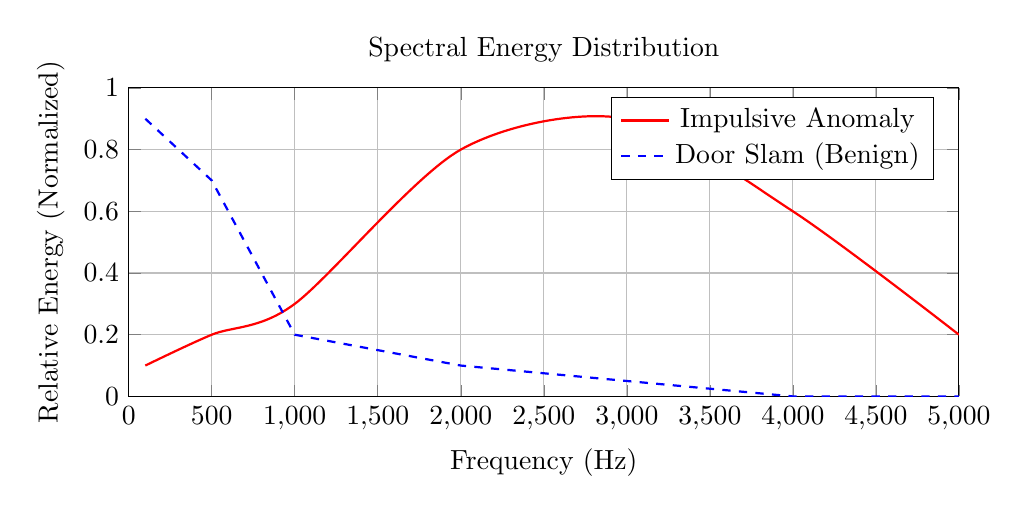
\begin{tikzpicture}
\begin{axis}[
    title={Spectral Energy Distribution},
    xlabel={Frequency (Hz)},
    ylabel={Relative Energy (Normalized)},
    xmin=0, xmax=5000,
    ymin=0, ymax=1,
    legend pos=north east,
    grid=major,
    width=\columnwidth,
    height=5.5cm
]
\addplot[color=red, thick, smooth] coordinates {
    (100,0.1)(500,0.2)(1000,0.3)(2000,0.8)(3000,0.9)(4000,0.6)(5000,0.2)
};
\addlegendentry{Impulsive Anomaly}

\addplot[color=blue, thick, dashed] coordinates {
    (100,0.9)(500,0.7)(1000,0.2)(2000,0.1)(3000,0.05)(4000,0.0)(5000,0.0)
};
\addlegendentry{Door Slam (Benign)}
\end{axis}
\end{tikzpicture}
\caption{Spectral Discrimination Profile. Impulsive anomalies (Red) exhibit high energy in the 2-4kHz range, while physical impacts (Blue) are dominated by low frequencies, forming the physical basis for the $\delta$ discrimination index.}
\label{fig:spectral}
\end{figure}

% ==========================================
% VII. DISCUSSION
% ==========================================
\section{Discussion}

The experimental results highlight several practical tradeoffs associated with deploying deterministic acoustic sensing in reverberant environments.

\subsection{Acoustic Robustness versus Semantic Richness}
The proposed AED system, in contrast to transformer-based systems, does not rely on higher-order semantics for classification. In real-time edge safety applications, the precise labeling of events is less important than timely, deterministic location. The use of semantic models adds additional latency due to buffering and increases memory requirements, which violate the requirement of sub-150 milliseconds. The proposed layered filter using spectral and periodic rejection provides stability in the alerts while maintaining deterministic latency.

\subsection{Privacy by Architectural Constraint}
Continuous acoustic sensing frequently encounters privacy objections \cite{b4, b33}. The proposed architecture addresses this through structural processing restrictions rather than policy enforcement alone.

PCM audio is loaded into a bounded RAM buffer and is immediately overwritten after feature extraction. There is no conversion to speech-to-text or any form of audio storage. The module generates only minimal directional metadata:
\begin{equation}
[\texttt{TIMESTAMP, ANOMALY\_CONFIDENCE, AZIMUTH\_ANGLE}]
\end{equation}

Such data reduction is in line with privacy principles within architecture \cite{b32}. The sensing node cannot interpret semantic exchanges, as the data are deterministically obfuscated. This design feature ensures scalability for operation; metadata data packets require little bandwidth usage, and can be extensively deployed without congesting the network infrastructure.

\subsection{Limitations}
The evaluation exposes several physical and architectural limitations inherent to the proposed framework:
\begin{itemize}
    \item \textbf{Corridor-Specific Thresholding:} Periodic and spectral thresholds ($\rho$, $\delta$) have been optimized for the reflective surface characteristics of institutional corridor environments; changes in absorptive conditions, occupancy-related reverberation time, or HVAC system operational variations would necessitate adjustment.
    \item \textbf{Azimuth-Only Localization:} Linear microphone array localizes only along the azimuth. Volumetric arrays are required in multi-layered environments for elevation determination. The vibration effect caused by mounting on the ceiling or aging of microphones may disturb the localization process.
    \item \textbf{Reverberant Drift and Multi-Source Overlap:} While GCC-PHAT mitigates multipath smearing, multi-source overlap conditions and metallic reflection artifacts can still induce angular drift ($\pm 8^{\circ}$).
    \item \textbf{Crowd-Noise Masking:} Dense crowd chatter masks the 2--4 kHz impulse band, degrading recall under 70 dB ambient conditions.
    \item \textbf{Absence of Semantic Intent:} The pipeline detects physical impulses but cannot interpret semantic intent or context, making it strictly a deterministic anomaly detector.
\end{itemize}

% ==========================================
% VIII. CONCLUSION
% ==========================================
\section{Conclusion}
The experiment proved that deterministic signal processing chains could effectively recognize impulsive NLOS events within a reverberant corridor environment with bounded latency and bounded retention properties intact. Through spectral discrimination based on the STFT, periodic rejection via autocorrelation analysis, and GCC-PHAT location determination, the acoustic processing component recognizes impulsive events in an officially defined reverberant operation domain.

Assessment revealed that, given the tested corridor environment, detection accuracy surpasses 95\% within a 15m NLOS safety range. With an operation within a tight memory range, along with the immediate overwriting of the raw audio input, latency remains less than 120ms. Although there is a reduction in the recall capability during high chatter SNR, the system can mitigate periodic mechanical noise.

With regard to the larger ScholarMaster framework, this architecture can serve solely as a deterministic sub-system for detecting sounds using acoustics—abstracting space-based information but without enacting any privacy policies or implementing any activation governance structure . It is utilized only for detecting acoustic events and calculating metadata based on their directionality.

% ==========================================
% REFERENCES
% ==========================================
\begin{thebibliography}{00}

\bibitem{b20} C. Knapp and G. Carter, ``The generalized correlation method for estimation of time delay,'' \textit{IEEE Transactions on Acoustics, Speech, and Signal Processing}, vol. 24, no. 4, pp. 320-327, 1976.

\bibitem{b30} J. B. Allen and D. A. Berkley, ``Image method for efficiently simulating small-room acoustics,'' \textit{The Journal of the Acoustical Society of America}, vol. 65, no. 4, pp. 943-950, 1979.

\bibitem{b9} J. Blauert, \textit{Spatial Hearing: The Psychophysics of Human Sound Localization}, MIT Press, 1997.

\bibitem{b27} J. H. DiBiase, ``A high-accuracy, closed-form approximation to the equivalency between SRP-PHAT and TDOA,'' in \textit{Proc. IEEE ICASSP}, 2000.

\bibitem{b31} H. Fastl and E. Zwicker, \textit{Psychoacoustics: Facts and Models}, Springer Science \& Business Media, 2006.

\bibitem{b1} A. Cavallaro, ``Privacy in video surveillance,'' \textit{IEEE Signal Processing Magazine}, vol. 24, no. 2, pp. 168-169, 2007.

\bibitem{b5} G. Valenzise, L. Gerosa, M. Tagliasacchi, F. Antonacci, and A. Sarti, ``Scream and gunshot detection and localization for audio-surveillance systems,'' in \textit{2007 IEEE Conference on Advanced Video and Signal Based Surveillance}, pp. 21-26, 2007.

\bibitem{b28} H. Kuttruff, \textit{Room Acoustics}, 5th ed. CRC Press, 2009.

\bibitem{b32} A. Cavoukian, ``Privacy by Design: The 7 Foundational Principles,'' \textit{Information and Privacy Commissioner of Ontario}, 2009.

\bibitem{b25} P. A. Naylor and N. D. Gaubitch, \textit{Speech Dereverberation}, Springer, 2010.

\bibitem{b33} J. H. Ziegeldorf, O. G. Morchon, and K. Wehrle, ``Privacy in the Internet of Things: threats and challenges,'' \textit{Security and Communication Networks}, vol. 7, no. 12, pp. 2728-2742, 2014.

\bibitem{b12} D. Barchiesi, D. Giannoulis, D. Stowell, and M. D. Plumbley, ``Acoustic scene classification: Classifying environments from the sounds they produce,'' \textit{IEEE Signal Processing Magazine}, vol. 32, no. 3, pp. 16-34, 2015.

\bibitem{b16} N. D. Lane et al., ``DeepX: A Software Accelerator for Low-Power Deep Learning Inference on Mobile Devices,'' in \textit{IPSN}, 2016.

\bibitem{b2} M. Crocco, M. Cristani, A. Trucco, and V. Murino, ``Audio surveillance: A systematic review,'' \textit{ACM Computing Surveys}, vol. 48, no. 4, pp. 1-46, 2016.

\bibitem{b26} W. Shi, J. Cao, Q. Zhang, Y. Li, and L. Xu, ``Edge Computing: Vision and Challenges,'' \textit{IEEE Internet of Things Journal}, vol. 3, no. 5, pp. 637-646, 2016.

\bibitem{b8} T. Virtanen, M. D. Plumbley, and D. Ellis, \textit{Computational Analysis of Sound Scenes and Events}, Springer, 2018.

\bibitem{b15} J. Chen and X. Ran, ``Deep Learning With Edge Computing: A Review,'' \textit{Proceedings of the IEEE}, vol. 107, no. 8, pp. 1655-1674, 2019.

\bibitem{b22} Q. Kong et al., ``PANNs: Large-scale Pretrained Audio Neural Networks for Audio Pattern Recognition,'' \textit{IEEE/ACM Transactions on Audio, Speech, and Language Processing}, vol. 28, pp. 2880-2894, 2020.

\bibitem{b23} Y. Gong, Y.-A. Chung, and J. Glass, ``AST: Audio Spectrogram Transformer,'' in \textit{Proc. Interspeech}, 2021, pp. 571-575.

\bibitem{b4} S. Gharib, M. Tran, D. Luong, K. Drossos, and T. Virtanen, ``Adversarial representation learning for robust privacy preservation in audio,'' \textit{IEEE Open Journal of Signal Processing}, vol. 5, pp. 294--302, 2024.

\bibitem{b34} P. Narendra et al., ``Memory-Bound Edge Efficiency Envelope (MBEEE): A Hardware-Level Analytical Model,'' \textit{Journal for Basic Sciences}, vol. 26, no. 5, pp. 31--37, 2026.

\bibitem{b10} S. Mallat, \textit{A Wavelet Tour of Signal Processing: The Sparse Way}, 3rd ed. Academic Press, 2008.

\bibitem{b11} L. Rabiner and B. Juang, \textit{Fundamentals of Speech Recognition}. Prentice Hall, 1993.

\bibitem{b19} E. Fonseca, X. Favory, J. Pons, F. Font, and X. Serra, ``FSD50K: An Open Dataset of Human-Labeled Sound Events,'' \textit{IEEE/ACM Transactions on Audio, Speech, and Language Processing}, vol. 30, pp. 829-852, 2021.

\bibitem{b21} M. Gruteser and D. Grunwald, ``Anonymous usage of location-based services through spatial and temporal cloaking,'' in \textit{Proceedings of the 1st International Conference on Mobile Systems, Applications and Services (MobiSys)}, 2003, pp. 31-42.

\bibitem{b29} J. Benesty, J. Chen, and Y. Huang, \textit{Microphone Array Signal Processing}. Springer Science \& Business Media, 2008.

\bibitem{b35} S. Hershey et al., ``CNN architectures for large-scale audio classification,'' in \textit{2017 IEEE International Conference on Acoustics, Speech and Signal Processing (ICASSP)}, 2017, pp. 131-135.
\end{thebibliography}

\end{document}